%06/05 - Carlos Aguirre
\chapter{Grafos aleatorios, grafos regulares y redes de mundo pequeño}
\section{Grafos aleatorios}
\subsection{Modelo de Erdös y Rényi}
En las redes reales muy raramente suele aparecer una topología aletoria. Sin embargo los grafos aleatorios han sido muy estudiados por las siguientes razones. Si encontramos una propiedad que ocurre con probabilidad 1 para ciertos parámetros de la red, podemos saber si nuestra red tiene esa propiedad solo con mirar sus parámetros. Para predecir el comportamiento de ciertas propiedades en función de parámetros de la red. Para comprobar si nuestra red tiene sesgos estructurales.

El modelo de Erdös y Rényi  se estudió en los años 50-60. Cada rama del grafo existe con una probabilidad p, que suele seguir una distribución uniforme.

Otra forma de definir los grafos aleatorios es seleccionar parejas de nodos aleatoriamente. Se seleccionan exactamente $pN(N-1)/2$ parejas. Ambos tipos de grafos aleatorios son equivalentes.

\subsection{Propiedades}
El estudio de grafos aleatorios se centra sobre todo en averiguar para que probabilidad p aparece cierta propiedad Q:
\begin{itemize}
\item Cuando el grafo es conexo.
\item Cuando la distancia media es menor que cierto número.
\item Cuando el índice de clusterización es mayor que cierto número.
\end{itemize}

Erdös y Rényi descubrieron que las propiedades Q aparecían de forma repentina según crecía p. Para muchas propiedades Q se verifica que existe una \textbf{probabilidad crítica} $p_c(N)$ tal que:
\begin{itemize}
\item Con probabilidad 0 el grafo no tiene Q si $p(N) < p_c(N)$
\item Con probabilidad 1 el grafo tiene Q si $p(N) > p_c(N)$
\end{itemize}

\subsection{Subgrafos}
La primera propiedad que estudiaron fue la aparición de subgrafos. Por ejemplo, a que probabilidad crítica p casi todo grafo G contiene un árbol de orden 3. 
La probabilidad crítica $p_c(N)$ de encontrar algunos subgrafos es:
\begin{figure}
\centering
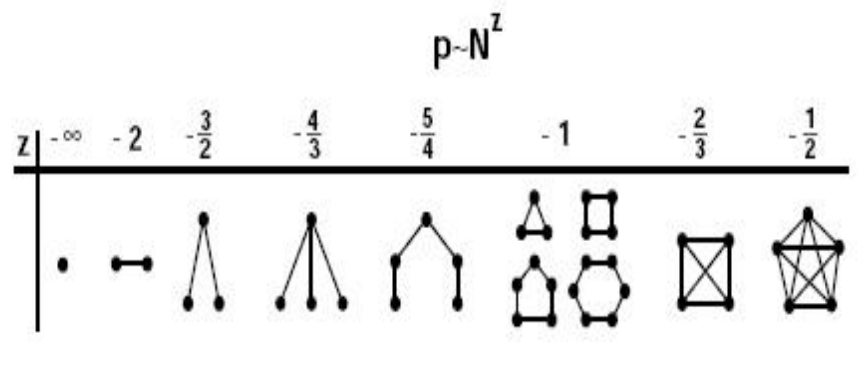
\includegraphics[width = 0.7\textwidth]{figs/prob-critica.png}
\end{figure}

Ejercicio: Calcular la probabilidad crítica p para que una red aleatoria de 1000 nodos contenga tanto un ciclo de orden 5 como un cliqué de orden 5 (cuidado, tiene truco).
\marginpar[\footnotesize Pregunta examen antigua] \
El ciclo de orden 5 aparece con una Z de -1
Un cliqué de 5 aparece con una Z de -0.5. 
Para que haya un cliqué de orden 5 es obligatorio que haya un ciclo de orden 5. Por tanto, teniendo N = 1000 nodos, solo habría que calcular la probabilidad de un cliqué: $1000^{-1/2} = 0.031$.

\subsection{Clusters}
Un subgrafo aislado y conexo es un
cluster. Erdös y Rényi demostraron que la estructura de clusters de un grafo
cambia abruptamente cuando el grado medio (número de ramas dividido entre el número de nodos) se acerca a 1.
$$\langle k \rangle = \frac{\frac{N \cdot (N-1)}{2} \cdot p}{N} = \frac{p \cdot (N-1)}{2} \xrightarrow{N \to \infty} p\frac{N}{2}$$

Si el grado medio <k> está entre 0 y 1, casi todos los clusters son árboles (en su mayor parte) o clusters que contienen un solo ciclo. El número de clusters es de orden N-n (número de nodos menos número de ramas), y el cluster mayor es un árbol de tamaño proporcional a N. 

Si el grado medio <k> es mayor que 1, la estructura anterior cambia completamente. Aparece un cluster gigante con [1-f(<k>)]N nodos donde f es una función que decae exponencialmente de 1 a 0 cuando x va a infinito. Los demás clusters pertenecen a árboles con Nf(<k>) nodos.

\subsection{Distribución de grado}
El grado de cada nodo sigue una distribución binomial. La distribución del grado de los nodos sigue una distribución de Poisson. 

\subsection{Conexidad y diámetro}
El diámetro de un grafo es la máxima distancia entre cualquier par de nodos. Si p no es demasiado pequeño los grafos aleatorios tienden a tener poco diámetro. Casi todos los grafos aleatorios tienen el mismo diámetro (más o menos) para la mayor parte de los valores de p.

En general se tiene:
\begin{itemize}
\item Si $\langle k \rangle < 1$: el grafo tiene árboles aislados.
\item Si $\langle k \rangle > 1$: aparece el cluster gigante y el diámetro del grafo es el del cluster gigante. Para $\langle k \rangle > 3.5$, el diámetro es proporcional a $\ln(N)/\ln(<k>)$.
\item Si $\langle k \rangle \geq ln(N)$ : el grafo es conexo y su diámetro es próximo a $\ln(N)/\ln(\langle k \rangle)$
\end{itemize}

El camino característico se comporta de forma similar al diámetro. En particular:
 $$\ell_{rand} \sim \frac{\ln(N)}{\ln(\langle k \rangle)}$$
 
\subsection{Índice de clusterización}
En un grafo aleatorio la probabilidad de que dos vecinos de un nodo dado están conectados es igual a la que dos nodos elegidos al azar estén conectados.
\marginpar[\footnotesize Pregunta típica de examen] \
El índice de clusterización de un grafo alteatorio es p, la probabilidad de existencia de cada rama.

\section{Grafos regulares}
Son los mejor conocidos de forma analítica debido a sus simetrías. Existen expresiones cerradas para todas las métricas. Son los más usados en modelos de redes neuronales artificiales. También se usan como sustrato inicial para la generación de otros tipos de redes.

Un caso particular de grafos regulares son las mallas (grids) donde cada nodo se conecta a sus $2^d \cdot k$ vecinos más próximos, donde d es la dimensión del grid.

En las mallas monodimensionales, el índice de clusterización es de 0.75, el camino característico es $|V|/\langle k \rangle$, y la distribución del grado de los nodos es una delta en el valor $\langle k \rangle$. Es decir tanto L como C son más grandes de lo que correspondería en el grafo aleatorio equivalente y la distribución de grado se puede ver como el límite cuando la varianza tiende a 0.

%08/05 - Carlos Aguirre
\section{Redes de mundo pequeño}
En 1998 Watts y Strogatz (Nature, 1998) proponen un modelo de red dependiente de un parámetro p, que es distinto al parámetro p de las redes aleatorias. 
\marginpar[\footnotesize Buena pregunta de 1 punto] \
En redes aleatorias, significa la existencia de las ramas, pero aquí es la probabilidad de reasignación o recolocación de cada una de las ramas que ya tiene el grafo. 
 Este modelo interpola entre un grafo regular y un grafo aleatorio. Se colocan inicialmente los nodos en un anillo y cada nodo se conecta con los 2k vecinos a izquierda y derecha.

Para cada rama de este grafo, con probabilidad p se decide si la rama se modifica o no.
Si la rama se modifica, se elige un nuevo nodo al azar con probabilidad uniforme. Se evitan ramas dobles y autoconexiones. Este proceso produce pNk atajos en el grafo.

\begin{figure}[h]
\centering
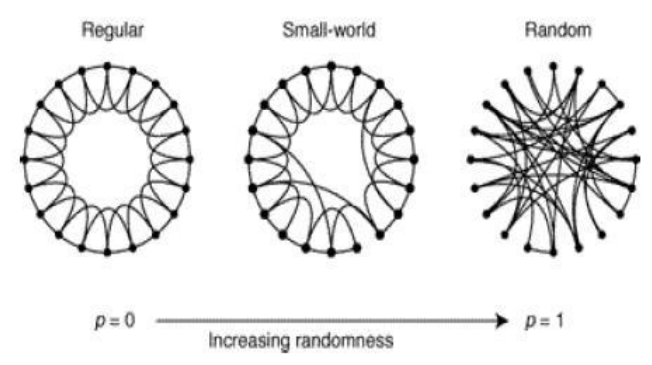
\includegraphics[width = 0.5\textwidth]{figs/grafos.png}
\end{figure}

El método de Watts y Strogatz puede producir grafos no conexos. Un método alternativo propuesto por Newman consiste en añadir de forma aleatoria un número pequeño de ramas sobre el sustrato inicial (duplicación y manteniendo la rama original).

\subsection{Sustrato inicial}
Como sustrato inicial se suele tomar un grid monodimensional cumpliendo las siguientes condiciones:
$$N \gg k \gg \log(N)$$
Cada nodo esta conectado con sus 2k vecinos a izquierda y derecha.

Así, el grafo siempre será conexo ($k \gg \log(N)$) y disperso ($N \gg k$). 

\subsection{Sustratos bi-conexos}
Un grafo conexo tiene un camino que une cualquier par de nodos. Una red biconexa es aquella que para cualquier par de nodos tiene al menos dos caminos que los unen. Por ejemplo, un anillo es una red biconexa porque se puede llegar por la izquierda y por la derecha. Las redes biológicas suelen ser biconexas, pero no todas lo son. Calcular tres o más caminos es un problema NP completo - buscar uno es fácil mediante un algoritmo en anchura y buscar dos se puede hacer con el algoritmo de Tarjan.

El modelo de red original de Watts y Strogatz tiene el mismo número de componentes biconexas que los grafos regulares. Las redes reales suelen tener un número mayor de componentes biconexas (p. ej. redes de comunicaciones o muchas redes biológicas).

Los grafos de mundo pequeño tienen el mismo índice de clusterización que un grafo aleatorio regular con el mismo número de ramas y nodos. Camino característico de un grafo aleatorio con el mismo número de nodos y ramas.

El modelo anterior permite crear redes de tipo Mundo-pequeño con un número elevado de componentes bi-conexas. El sustrato inicial es un grafo regular pero con un numero elevado de componentes biconexas. Presenta una transición a aleatorio similar a la de los anillos.

\subsection{Sustratos dirigidos y ponderados}
El modelo original de Watts y Strogatz no contempla la posibilidad de grafos con dirección y peso. Existen redes en la naturaleza donde aparecen la direccionalidad y el peso (redes neuronales, redes sociales, redes de interacción, etc).

\subsection{Parámetros}
El procedimiento de Watts y Strogatz sobre el sustrato inicial produce una transición en el comportamiento del camino característico y del índice de clusterización. Ambos dos han de pasar de valores altos propios del grafo regular a valores pequeños propios del grafo aleatorio.

En una malla monodimensional $L = O(N)$ y $C = O(1)$. En un grafo aleatorio: $L = O(\log(N))$ y $C = 0 = p$.

Watts y Strogatz observaron que la transición en el comportamiento de los valores era diferente para el
caso de camino característico L y para el índice de clusterización C. El camino característico presentaba la transición de régimen mucho antes que el índice de clusterización.

Cuando se consideran otros sustratos tales como grafos bi-conexos o grafos con dirección peso también se puede observar el mismo fenómeno en el comportamiento de C y L. Además las propiedades iniciales del grafo (bi-conectividad, dirección, peso) no se pierden durante la transición

L no empieza a decrecer hasta que $p > 1/Nk$ (es decir hasta que no aparece al menos un atajo). Por tanto, el valor de p para el cual se entra en la zona de mundo pequeño es dependiente de N y k. Para una probabilidad fija p, existe un valor N' tal que $L = O(N)$ si$ N < N'$ y $L=O(\log(N))$ sin $N > N'$. Se puede demostrar el valor de p que para un valor fijo de N y k produce la transición de L es $p = 1/kN$.

La distribución del grado de los nodos debe pasar de una delta (vale 1 en 0 y 0 en todos los demás) en el grado medio de cada nodo (2k) a una distribución de Poisson.

La distribución espectral (de la matriz de autovalores) también sufre una transición en función de p.